\documentclass{sigchi}

% Override default copyright strip
\toappear{Permission to make digital or hard copies of all or part of this work for personal or classroom use is granted without fee provided that copies are not made or distributed for profit or commercial advantage and that copies bear this notice and the full citation on the first page. Copyrights for components of this work owned by others than ACM must be honored. Abstracting with credit is permitted. To copy otherwise, or republish, to post on servers or to redistribute to lists, requires prior specific permission and/or a fee.}

% Load basic packages
\usepackage{balance}
\usepackage{graphics}
\usepackage{txfonts}
\usepackage{times}
\usepackage[pdftex]{hyperref}
\usepackage{color}
\usepackage{textcomp}
\usepackage{booktabs}
\usepackage{ccicons}
\usepackage{todonotes}
\usepackage{notoccite}

% Define a global style for URLs, rather that the default one
\makeatletter
\def\url@leostyle{%
  \@ifundefined{selectfont}{\def\UrlFont{\sf}}{\def\UrlFont{\small\bf\ttfamily}}}
\makeatother
\urlstyle{leo}

% To make various LaTeX processors do the right thing with page size
\def\pprw{8.5in}
\def\pprh{11in}
\special{papersize=\pprw,\pprh}
\setlength{\paperwidth}{\pprw}
\setlength{\paperheight}{\pprh}
\setlength{\pdfpagewidth}{\pprw}
\setlength{\pdfpageheight}{\pprh}

% Make sure hyperref comes last of your loaded packages, to give it a
% fighting chance of not being over-written, since its job is to
% redefine many LaTeX commands.
\definecolor{linkColor}{RGB}{6,125,233}
\hypersetup{%
    pdftitle={SIGCHI Conference Proceedings Format},
    pdfauthor={LaTeX},
    pdfkeywords={SIGCHI, proceedings, archival format},
    bookmarksnumbered,
    pdfstartview={FitH},
    colorlinks,
    citecolor=black,
    filecolor=black,
    linkcolor=black,
    urlcolor=linkColor,
    breaklinks=true,
}

\begin{document}

\title{AtmoSPHERE}

\numberofauthors{1}
\author{%
    \alignauthor{Jay Feng, William Hwang, Joseph Wu, Mingyu Zhang \\
        \affaddr{CSE 477, Spring 2015}} \\
}

\maketitle

\begin{abstract}
    Air quality is an upstream component of human health, which cannot be addressed through primary care health facilities.
    In this work, we present AtmoSPHERE, a connected, wearable air monitor.
    Our system is comprised of a wrist-worn sensor suite, a connected smartphone, and a cloud service.
    The sensor suite measures two major categories of airborne health risks: particulate matter and volatile organics.
    The phone tags the data with location data and is used to communicate between the sensors and cloud.
    From the cloud service, we display a dashboard to highlight air quality in travelled areas.
    To evaluate the system, we collected data from 2 users over the course of a week of normal activity.
\end{abstract}

\category{J.3}{Health}{}

\keywords{Air quality; Upstream health; Wearable; Connected devices; Distributed sensors.}

\section{Introduction}
% Background/Motivation
Approximately half of all known health conditions originate from environmental factors\cite{Manchanda:TEDTalk}.
These factors are generally labelled ``upstream'' factors due to how they are detached from a person's immediate symptoms during illness.
Upstream factors include variables such as the sanitation of a person's home, the condition of their workplace, or the local air.
The existing health care system is not equipped to handle issues outside the hospital or clinic.
However, many upstream factors are simple to identify, straight forward to address.
We envision a device that can inform the user and others in the vicinity about one subset of upstream health risks.

% PM sensor background
In this project, we introduce AtmoSPHERE, a wearable air monitor for both particulate matter and volatile organic compounds (VOC).
Particulate matter (PM), is any microscopic matter suspended in the atmosphere.
Particulates include dust as well as more dangerous varieties classified by their diameter in microns, known as PM10 and PM2.5.
A PM sensor is comprised of an infrared emitting diode and a phototransistor placed diagonally\cite{PMSensor:Datasheet}.
As particles pass through the path between the two components, deflected light is recorded by the phototransistor.
This approach can detect visible dust as well as finer particles, such as PM2.5.

% VOC sensor background
Volatile organic compounds (VOC) are compounds with high vapor pressure at room temperature.
VOCs are numerous and varied, and include harmful compounds such as benzene, chlorofluorocarbons, and methylene chloride.
A VOC sensor comes in many forms.
A semiconductor VOC sensor uses a chemical reaction between the air and a heated substrate, such as Tin Dioxide\cite{VOCSensor:Datasheet}.
As the concentration of VOC in the air increases, the corresponding resistance of the substrate drops by a measurable amount.

% Advantages of a wearable
AtmoSPHERE is intended to allow distributed sensing of environmental risks.
The wearable is linked to a smartphone and through that, our cloud service and data API.
By aggregating data from multiple users, we can build substantial maps of local air quality.
We expect this device can be used to inform lifestyle changes.

\section{Theory of Operation}
% How to wear it
The only physical requirement of the AtmoSPHERE is sufficient air flow through the device.
The wearable is designed to be worn on the wrist, where the movement of the arms will agitate air into the sensors.
However, the device can be attached to any other location on the body.
The wearable also doubles as a stationary air monitor, such as when taken off during charging.
While stationary, diffusion is also an acceptable means of passing air over the sensor.

% Phone companion
For data collection, the wearable should always be within a short distance of a paired Android phone.
The wearable and phone communicate via Bluetooth, so the maximum separation of the two devices should not exceed 10 meters.
At the same time, the phone should have location services enabled and at least an intermittent internet connection.

\section{Implementation Details}
Figure~\ref{fig:software block} shows the system architecture and data flow.
In this section, we will detail the hardware design, the software features, and the data API.
\begin{figure}
    \centering
    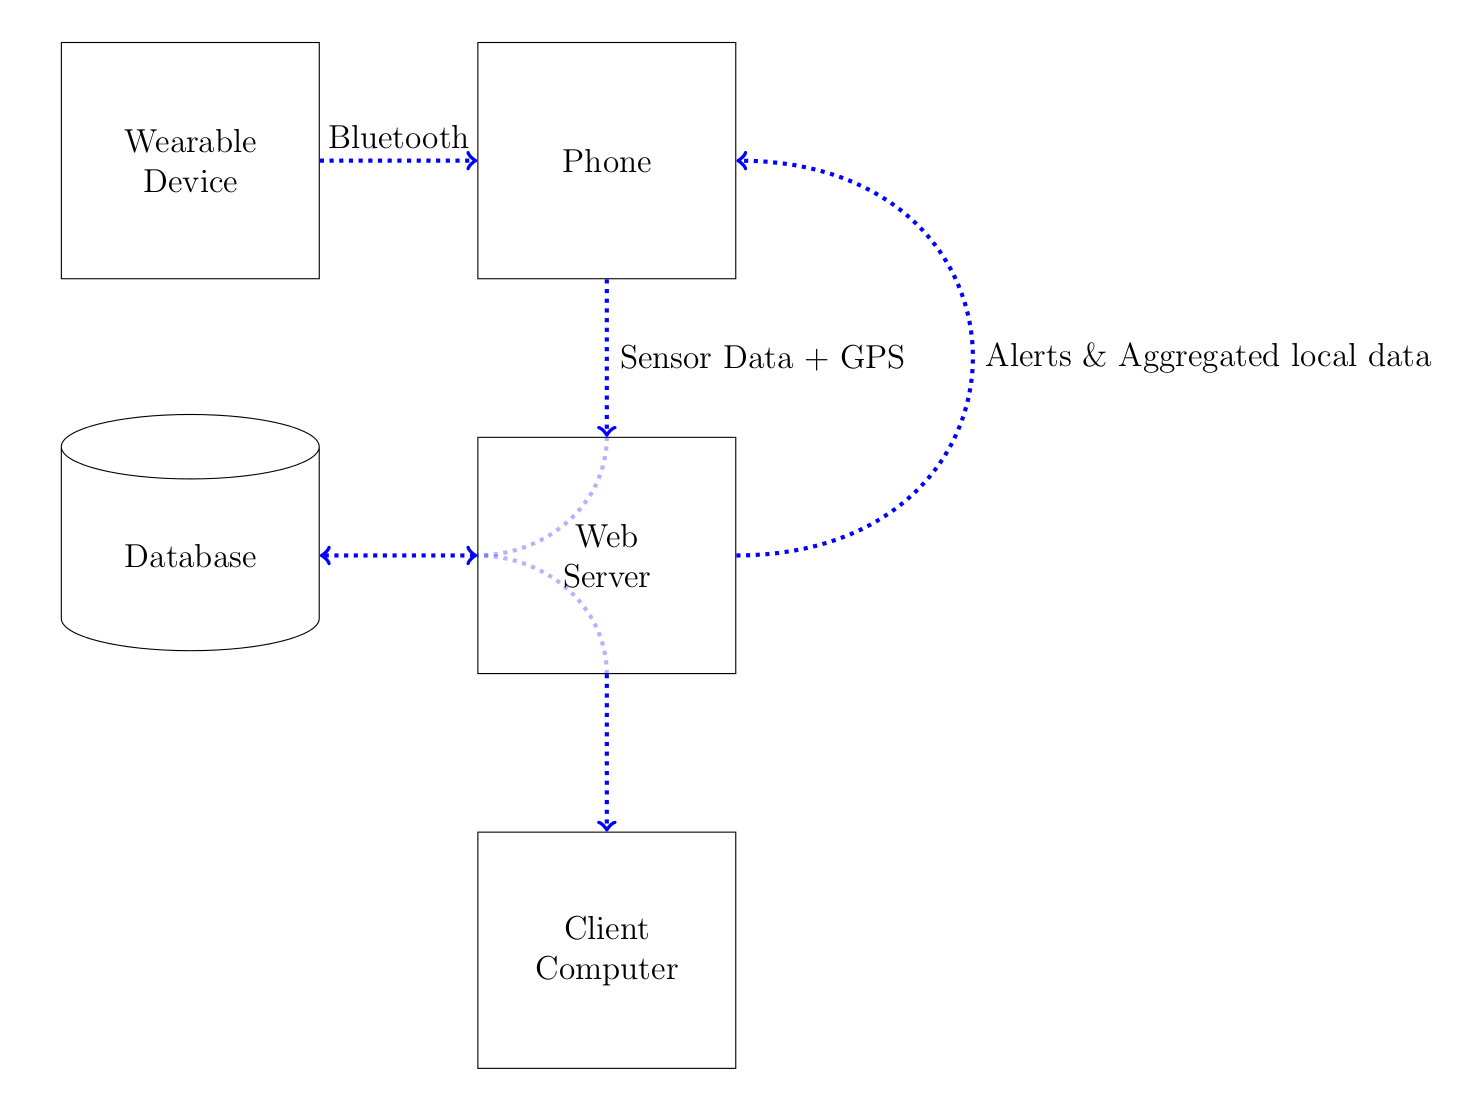
\includegraphics[width=0.9\columnwidth]{figures/Software-Block-Diagram.jpg}
    \caption{Insert a caption below each figure. Do not alter the Caption style.}
    ~\label{fig:software block}
\end{figure}

\subsection{Hardware}
TODO

\subsection{Phone Application}
TODO

\subsection{Web Application}
TODO

\subsection{Data API}
TODO

\section{Results}
TODO

\section{Challenges}
TODO

\section{Future Work and Discussion}
TODO

\section{Conclusion}
TODO

% Try to balance the columns of the last page
\balance{}

\bibliographystyle{SIGCHI-Reference-Format}
\bibliography{report}

\end{document}
